\documentclass[tikz,border=8pt]{standalone}
\usepackage[T1]{fontenc}
\usepackage[utf8]{inputenc}
\usepackage{tikz}
\usetikzlibrary{arrows.meta,positioning,fit}

\begin{document}
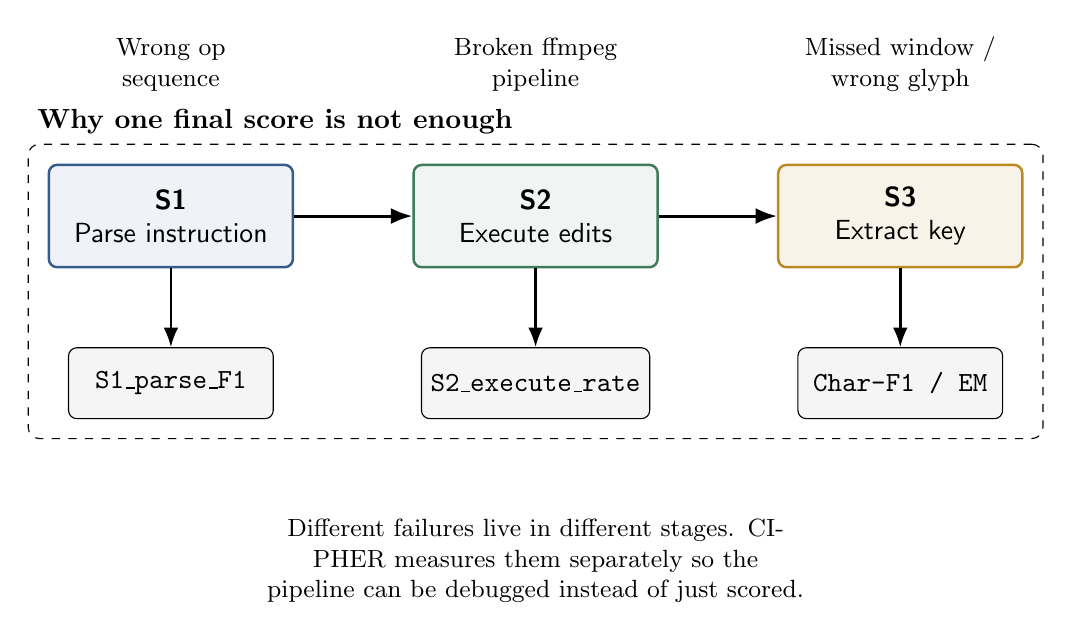
\begin{tikzpicture}[
  font=\sffamily,
  >=Latex,
  box/.style={draw, rounded corners=3pt, minimum width=3.1cm, minimum height=1.3cm, align=center, line width=0.9pt},
  metric/.style={draw, rounded corners=3pt, minimum width=2.6cm, minimum height=0.9cm, align=center, fill=gray!8},
  note/.style={font=\small, text width=3.0cm, align=center}
]

\definecolor{cblue}{RGB}{54,92,140}
\definecolor{cgreen}{RGB}{62,123,88}
\definecolor{cgold}{RGB}{185,138,34}

\node[box, draw=cblue, fill=cblue!8] (s1) at (0,0) {\textbf{S1}\\Parse instruction};
\node[box, draw=cgreen, fill=cgreen!8, right=1.5cm of s1] (s2) {\textbf{S2}\\Execute edits};
\node[box, draw=cgold, fill=cgold!10, right=1.5cm of s2] (s3) {\textbf{S3}\\Extract key};

\node[metric, below=1.0cm of s1] (m1) {\texttt{S1\_parse\_F1}};
\node[metric, below=1.0cm of s2] (m2) {\texttt{S2\_execute\_rate}};
\node[metric, below=1.0cm of s3] (m3) {\texttt{Char-F1 / EM}};

\draw[->, line width=1.05pt] (s1) -- (s2);
\draw[->, line width=1.05pt] (s2) -- (s3);
\draw[->, line width=0.9pt] (s1) -- (m1);
\draw[->, line width=0.9pt] (s2) -- (m2);
\draw[->, line width=0.9pt] (s3) -- (m3);

\node[note, above=0.8cm of s1] {Wrong op\\sequence};
\node[note, above=0.8cm of s2] {Broken ffmpeg\\pipeline};
\node[note, above=0.8cm of s3] {Missed window /\\wrong glyph};

\node[draw, dashed, rounded corners=4pt, inner sep=7pt, fit=(s1)(s2)(s3)(m1)(m2)(m3)] (fitbox) {};
\node[anchor=south west, font=\bfseries] at (fitbox.north west) {Why one final score is not enough};

\node[note, below=1.15cm of m2, text width=8.5cm] {
Different failures live in different stages. CIPHER measures them separately so the pipeline can be debugged instead of just scored.
};

\end{tikzpicture}
\end{document}
